\chapter{INTRODUCTION}
\label{chap:introduction}

\hs This chapter provides a general introduction to the host company of the Internship I in year 4 of department of \textbf{Applied Mathematics and Statistics (AMS)}, including its background, and key characteristics. It then narrows the focus to the specific problem addressed during the internship, with a clear definition of the project's objectives and scope. A chronological overview of the internship schedule is also presented, outlining major milestones as well as daily responsibilities. In addition, the primary tools and technologies employed throughout the project are described, along with their main features, and any constraints or regulatory requirements that influenced the work are examined. Recent work on aerial infrastructure inspection has highlighted the importance of robust multi-scale crack detection in UAV imagery.

\section{Presentation of Internship}
\subsection{Objective of Internship}
\hs Build an accurate, precise, and practically deployable AI model to detect and segment cracks presenting on
    large buildings, contributing to reduced infrastructural improvement, early maintenance and public safety.
    
    This project aims to design and validate a deep learning framework for automatic, pixel-level crack
    segmentation in high-resolution aerial imagery. Specific goals are to:

\begin{itemize}        
    \item Develop an empirical experiment on segmentation and detection models using modified Semantic Segmentation Models, Instance Segmentation models, and transformer-based models that are capable of capturing fine cracks on high-resolution images.
    \item Implement a tile-based inference pipeline with blended overlaps, allowing seamless processing of arbitrarily large-scale, high-resolution images on a single GPU.
    \item Evaluate the system on multiple real-world aerial crack datasets, including the CUBIT-InSeg large-scale UAV dataset \cite{10-zhao-2026-cubit-inseg}, comparing against published baselines.
\end{itemize}

\hs These objectives are pursued under a unified experimental protocol described in Chapter \ref{chap:methodology}, in which all models are trained on the same aggregated dataset and evaluated using the same metrics. Particular attention is given to the trade-off between segmentation accuracy and inference speed, since the final system is intended for deployment on inspection workstations with limited GPU memory.

\newpage

\subsection{Duration of Internship}

\hs The internship was carried out over a period of 3 months, commencing on \textbf{1 July 2026} and ending on \textbf{30 September 2026}. During this period, the internship was involved in research and development activities at Company's Engineer Lab.

This duration included activities such as defining the project, beginning with literature review and problem analysis, followed by implementation, testing, and evaluation of the proposed system. It also provided enough time to gain hands-on experience and adapt to the research and development environment.

\section{Presentation of Organization}

\subsection{General Information of the Organization}

\begin{figure}[H]
    \centering
    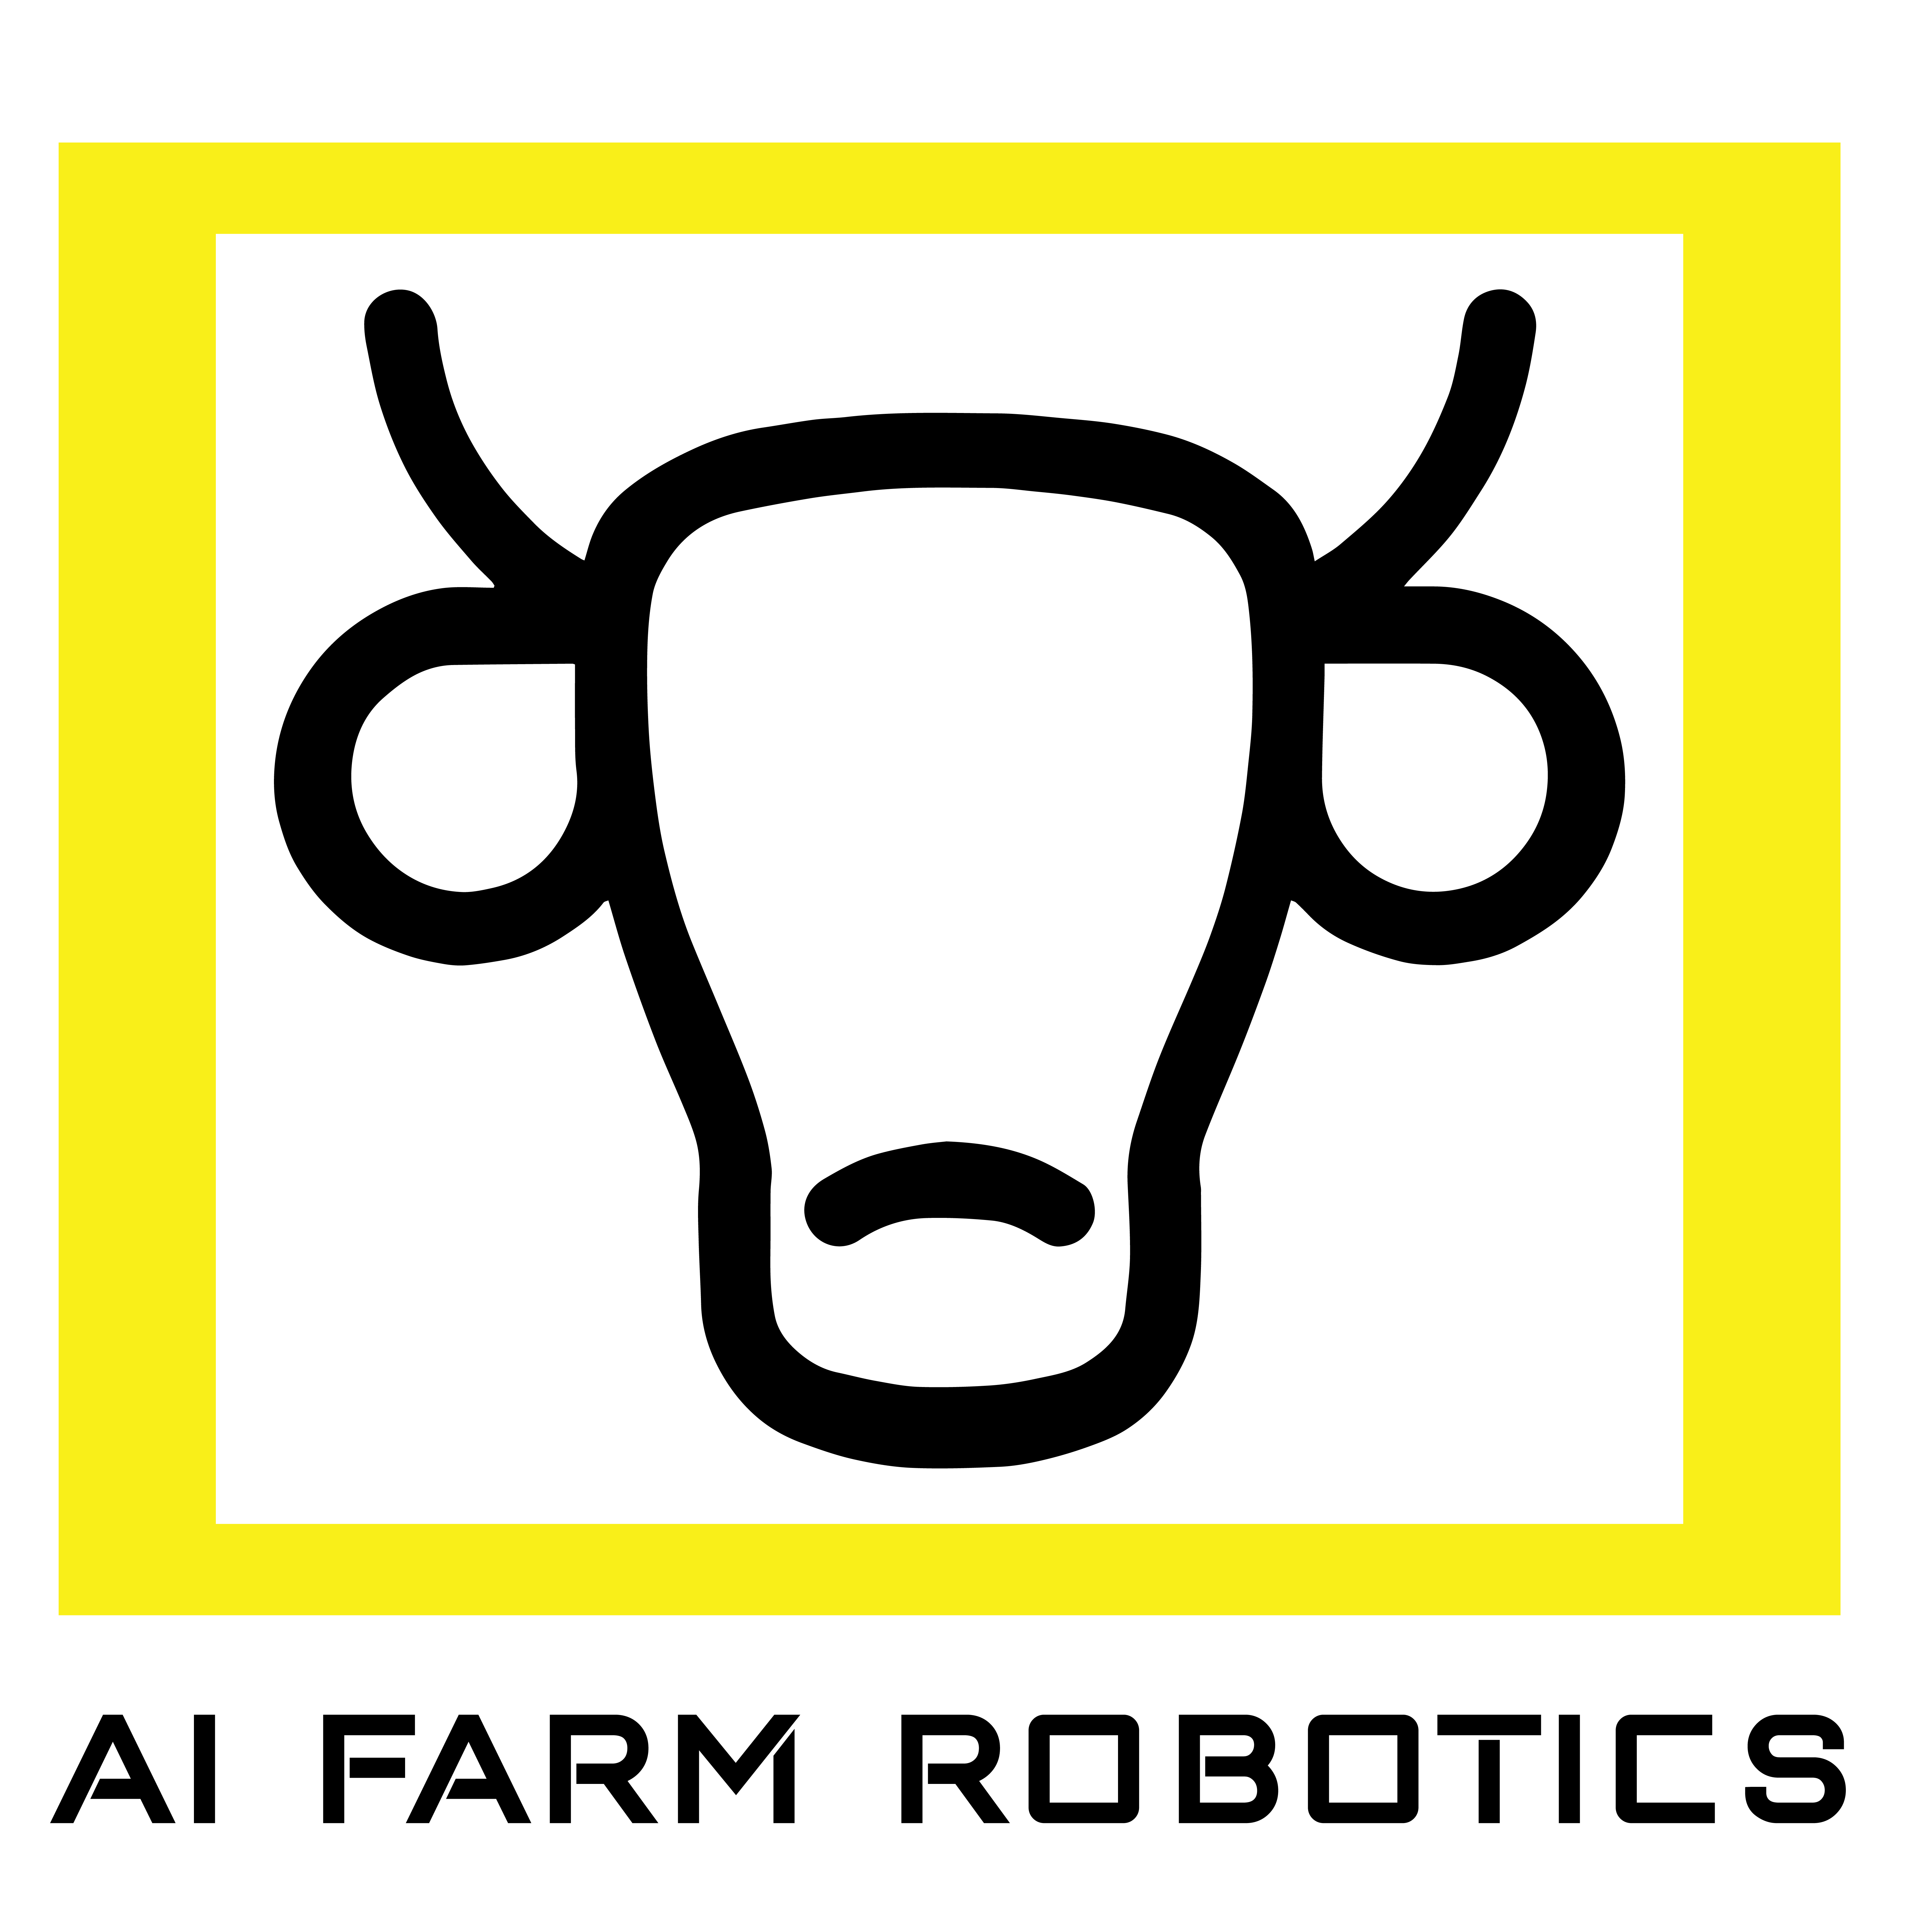
\includegraphics[width=0.3\textwidth]{figures/company/AI-FARM-Logo.png}
    \caption{\textit{AI Farm Robotics co. ltd.}}
    \label{fig:ai-farm-logo}
\end{figure}

\hs \textbf{AI Farm Robotics (AI Farm Co., Ltd.)} is a technology-driven robotics manufacturing company based in Phnom Penh, Cambodia. Operating as a subsidiary of the Khamsa Group of Businesses (KGB), the firm was founded to drive national technological sovereignty and transform Cambodia into a prominent robotics nation in Asia. The company's headquarters and primary research facility are located at \textbf{Connexion Building First Floor, Street Koh Pich, Sangkat Tonle Bassac, Khan Chamkar Mon, Phnom Penh, Cambodia}. From this hub, the company spearheads local innovation by specializing in the research and development of artificial intelligence, automated machinery, robot arms, mobile robots, drones, and tailored industrial automation systems.The company actively focuses on supporting micro, small, and medium enterprises (MSMEs) through flexible business models, including custom engineering, manufacturing, and Robot as a Service (RaaS) deployments. Beyond commercial production, AI Farm Robotics plays a vital role in national capacity building by running educational programs like the Robot Young Academy and dedicated STEM courses. These initiatives are designed to upskill the local workforce, prepare students for the digital economy, and close the technological gap in the region. By collaborating with domestic and international universities, trade organizations, and government bodies, the company continues to expand its technological portfolio and accelerate automated industrial adoption across Southeast Asia.

\subsection{Services and Functions of the Organization}
\label{subsec:services_and_functions_of_the_organization}

\hs \textbf{AI FARM Robotics} is an innovative technology and automation leading company based in Phnom Penh, Cambodia. The company specializes in artificial intelligence, robotics, and advanced engineering solutions tailored to modernize businesses. By combining local capacity building with cutting-edge technology, it helps micro, small, and medium enterprises (MSMEs) transition into automated environments. The company bridges the gap between complex technology and practical application through five core pillars of service:

\begin{itemize}        
    \item \textbf{Strategic Consulting:} Designing customized automation and AI strategies for local businesses and analyzing existing workflows to identify high-impact areas for robot implementation.
    \item \textbf{Engineering and System Integration:} Building and customizing physical robot frameworks and industrial components and installing and configuring automated machinery directly into business environments.
    \item \textbf{Software and AI Development:} Training intelligent models for data processing, computer vision, and predictive mechanics and developing localized, responsive algorithms and adaptive code creators for autonomous navigation.
    \item \textbf{Robot-as-a-Service (RaaS):} Providing operational service robots on a subscription or utility basis to lower upfront costs and deploying specialized automated cooking assistants, barista bots, and indoor delivery units.
    \item \textbf{Education and Capacity Building:} Offering STEM-focused courses, workshops, and training programs to cultivate a skilled workforce in robotics and AI and partnering with universities to provide hands-on learning experiences for students.
\end{itemize}

\subsection{Vision and Mission}

\textbf{Vision:} To become a leading robotics and AI company in Southeast Asia, driving technological innovation and empowering businesses to embrace automation.

\textbf{Mission:} To provide cutting-edge robotics and AI solutions that drive efficiency, productivity, and growth for businesses in Cambodia and beyond.

\subsection{Address and Contact}

\begin{itemize}        
    \item \textbf{Organization Name:} AI Farm Robotics Co., Ltd.
    \item \textbf{Website:} \href{https://aifarm.dev/}{aifarm.dev}
    \item \textbf{Email:} \href{mailto:info@aifarm.dev}{info@aifarm.dev}
\end{itemize}

\subsection{Internship Working Schedule}

\hs During the internship, AI FARM Robotics provided a full-time schedule for interns. The schedule assigned full-time sessions throughout the weekdays, allowing the workspace to be used efficiently.

Interns were expected to follow a fixed working schedule. For interns conducting their internship at AI FARM Robotics, the expected working hours were from \textbf{8:00 AM to 12:00 PM} and from \textbf{1:00 PM to 5:00 PM}.

In addition to the regular working schedule, a weekly progress meetings were held every \textbf{Friday from 9:00 AM to 12:00 PM} to report progress to the supervisor. These sessions provided an opportunity to present ongoing work, discuss challenges, receive feedback, and review the next steps of the project.

\section{Presentation of Project}

\subsection{Project Overview}

\hs This project aims to develop a robust and deployable deep learning framework for the automatic detection and pixel-level segmentation of cracks in large-scale, high-resolution aerial imagery captured by UAVs. The core challenge lies in overcoming the limitations of current models, which struggle to balance the detection of fine, thread-like cracks (often as thin as 1-3 pixels) with maintaining the global context of massive images (up to >50 megapixels).

To achieve this, the project will conduct empirical experiments using a range of advanced models, including semantic segmentation architectures (U-Net), instance segmentation models (YOLO), and transformer-based models (SegFormer, Swin Transformer), to identify the most effective approach. A key innovation of the project is the design and implementation of a tile-based inference pipeline with blended overlaps, which will enable the seamless processing of arbitrarily large images on a single GPU. To ensure robustness and real-world applicability, the model will be trained and validated on a diverse collection of public crack datasets and further fine-tuned on a custom dataset of high-resolution UAV images. The system's performance will be rigorously assessed using standard segmentation metrics like IoU, Precision, Recall, and F1-Score, with a final goal of creating an accurate and efficient tool for routine infrastructure inspection that can contribute to improved public safety and proactive maintenance.

\subsection{Problem Statement}
\hs Routine inspection of critical infrastructure, including bridges, buildings, and runways, is essential for public safety. However, current manual inspection methods are expensive (averaging \$X per mile), subjective, and limited in coverage. While AI-based crack detection has shown promise on close-up images (typically $< 5$ megapixels), applying these methods to aerial imagery introduces severe challenges. When a UAV captures a building facade from 15m altitude, a structural crack just 2mm wide is resolved as only 1--3 pixels in the 100+ megapixel image-occupying less than 0.01\% of the total area. Furthermore, the massive image size exceeds the memory limits of standard GPUs (typically 8--24GB VRAM), requiring specialized inference strategies. Current models fail to balance the preservation of these fine spatial details with global contextual understanding, and lack efficient gigapixel-scale inference pipelines.

\subsection{Objectives}

\hs Build an accurate, precise, and practically deployable AI model to detect and segment cracks presenting on large buildings, contributing to reduced infrastructural improvement, early maintenance and public safety. Furthermore, this project aims to design and validate a deep learning framework for automatic, pixel-level crack segmentation in high-resolution aerial imagery. Specific goals are to:

\begin{itemize}        
    \item Develop an empirical experiment on segmentation and detection models using modified Semantic, Segmentation Models, Instance Segmentation models, and transformer-based models that are capable of capturing fine cracks on high-resolution images.
    \item Implement a tile-based inference pipeline with blended overlaps, allowing seamless processing of arbitrarily large-scale, high-resolution images on a single GPU.
    \item Evaluate the system on multiple real-world aerial crack datasets, comparing against published baselines.
    \item Conduct a comprehensive performance analysis using standard segmentation metrics such as Intersection over Union (IoU), Precision, Recall, and F1-Score to quantify the model's effectiveness in detecting and segmenting cracks.
\end{itemize}

\subsection{Schedule of Internship}

\begin{figure}[H]
    \centering
    
\includegraphics[width=\textwidth]{figures/schools/schedule.png}
    \caption{\textit{Internship schedule}}
    \label{fig:internship-schedule}
\end{figure}